% !TeX root = ../thuthesis-example.tex

\chapter{相关研究综述}

\section{分布式系统故障}

系统组件故障是现代分布式系统普遍存在的问题。导致系统组件故障产生的原因众多,包括软件缺陷和硬件故障等,例如进程崩溃、磁盘损坏、程序错误会导致单一组件失效,网络延迟和分区可能导致系统组件的连接和通信出现故障,从而产生级联的连锁反应。系统组件故障的频率不容忽视。通常来讲,系统单一组件发生故障的时间间隔服从指数分布,多个组件之间的故障时间间隔相互独立,从而导致在大型分布式系统中故障的频率很高。根据谷歌的相关研究\cite{beyer2016site}, 每年会有超过1/100的机器出现内存崩溃,在百台节点组成的计算机集群,每一亿个小时会出现五千次左右的故障。

根据系统组件故障的产生原因,我们可以将分布式系统故障划分为以下几种类别\cite{michaud20062}:

1. 外部环境导致的故障。该故障产生的原因为不受控制的系统外部环境,例如机房停电、电缆断裂、火灾、地震海啸和其他自然灾害等。这种类型的故障无法通过分布式系统自身来自动解决和恢复,通常需要系统的搭建者通过在多个分散的地理位置部署数据和服务的副本来避免系统的中断和业务的损失。

2. 系统硬件失效导致的故障。该故障产生的原因为系统中一个或多个硬件不再正常工作,例如磁盘写满、内存不足、网络延迟等。这种类型的故障通常是高可用方案的重点解决对象,通过多副本、自动容错机制可以有效地减少这种故障对系统的实际影响。

3. 系统软件异常导致的故障。该故障产生的原因为应用程序在运行时出现偏离预期的行为,例如在缓冲区的边界之外写入数据导致内存损坏和进程崩溃、除零错误、返回值错误等。该问题通常不易解决,但是高可用方案可以为这类错误提供一定的容错和兜底。

4. 外部恶意攻击导致的故障。该故障产生的原因为人为恶意行为,例如例如代码注入攻击和ddos攻击等。该类故障通常通过专门的安全防御解决,但高可用方案方案依然可以在ddos等部分攻击场景下提供帮助,例如通过负载均衡的能力重新分配资源,从而让系统部分节点在遭受攻击和崩溃时依然能够提供服务。

本文提出的高可用方案的目标是“部分失效、整体可用”。具体而言,即使出于上述的任何原因系统内有部分组件出现故障,只要系统剩余存活的组件满足可用标准、资源足够、能够协同工作,那么系统就可以通过故障检测、自动容错、自动恢复等高可用机制保证服务的正常运行,降低错误在用户侧的感知,保证业务的连续性。

具体而言,本文提出的高可用方案能能够解决Kola\cite{kola2005faults}等人提出的分布式系统错误,包括以下具体问题:

1. 进程宕机,一些进程长时间甚至无限期地挂起,无法响应外部的请求。从请求方的角度来看,没有简单的方法来确定进程是否还在提供服务或是已经无法响应,

2. 磁盘空间不足。在数据暂存和写入期间,磁盘空间不足。

3. 硬件/软件/网络中断。间歇性网络中断、由服务器/客户端机器崩溃引起的中断以及用于硬件/软件升级和错误修复的停机时间导致在此期间的相关任务、RPC请求全部失效。

4. 资源过度消耗。由于并发数量过多、内存资源支出太多导致服务器崩溃,或是引发大量抖动导致传输效率降低、各种任务超时。


\section{高可用方案}

根据Ledmi\cite{ledmi2018fault}等人的相关研究,常见的高可用容错方案根据性质可以分为两大类,反应式容错(Reactive Fault Tolerance)和主动式容错(Proactive Fault Tolerance)。其中,反应式容错指的是系统在发生故障之后采取措施进行恢复,通常的步骤包括检测故障、诊断原因、系统恢复。而主动式容错指的是在系统发生故障之前就采取预防措施,预防故障的发生或减轻故障的影响。通常的步骤包括预测故障、预防故障、提前进行容错设计。

「这里应该插入一张图」

反应式容错技术通常用于降低系统在发生故障时产生的不良影响,包含重试(Retry)、复制(Replication)、检查点(Check-pointing)和消息日志(Message Logging)等相关技术。

1. 重试(Retry): 最常用的故障恢复技术。通过重试,期待系统能够在一段时间后自动恢复,从而实现故障恢复。

重试可以有效应对非永久性的瞬时故障,例如网络抖动、短暂的资源过载等问题,提高系统的可用性。同时由于分布式环境各种组件之间的交互复杂,故障难以避免,重试能够增强系统的整体鲁棒性,最大化进行自动的故障恢复,减少人工的干预和人力的投入。

根据不同的策略,重试可以分为立马重试、固定间隔等待重试、指数退避重试、随机退避重试和基于策略的重试方法。立马重试和固定间隔等待重试的实现简单,适用于预期故障能够快速恢复的场景,然而会给系统增加负载。
为了降低指数对于系统负载的影响,指数退避重试的思想是通过每次重试之间的时间间隔呈指数增长,有效缓解因频繁重试造成的系统压力,适用于故障恢复时间不确定的场景。
随机退避重试是在指数退避的基础上,增加随机抖动,避免大量客户端同时重试,造成雪崩效应。

基于状态的重试则是服务的提供方根据对自身的状态评估而给出一个重试建议,需要请求的双方提前约定好不同的错误状态的含义和重试的策略,从而提高重试的有效性。


2. 复制(Replication):通过为数据或者进程创建多个副本,并运行在独立的机器上,在某个副本失效的情况下,其他副本可以Failover并且完成任务。

单一数据意味着单点故障,往往通过引入冗余、为一份数据维护多副本的方式实现系统的可用性,
系统可以容忍特定数量的副本失效的错误,使用未失效的副本继续提供读写服务。
然而,多副本在带来系统可用性提升的同时,引入了数据一致性的问题。
共识协议旨在维护多份数据副本的一致性,使得在应用程序的角度上,多份数据副本看起来是一个统一的整体。
根据副本拓扑结构,共识协议可以分成单一领导者、多领导者、无领导者结构。
根据数据一致性分类,共识协议可以分成线性一致性\cite{herlihy1990linearizability}、顺序一致性\cite{attiya1994sequential}、最终一致性\cite{bailis2013eventual}。最终一致性中可以继续细化为因果一致性\cite{lloyd2011cops}、会话一致性\cite{mortazavi2018session}、读己之写一致性\cite{nishtala2013memcached}。

目前主流的共识协议中,Paxos\cite{lamport2001paxos}基于无领导拓扑结构实现了线性一致性语义。Paxos中的节点可以分成Proposer、Acceptor、Learner,通过两阶段协议实现多副本共识。第一阶段为准备阶段,由Proposer读取最新的值和版本,并且在Acceptor上预定下一次写入的Lease。第二阶段为接受阶段,由Acceptor决定是否接受本次Proposer的写入。Paxos协议在工业界有广泛应用,例如Google Chubby\cite{burrows2006chubby}和Google Spanner\cite{corbett2013spanner},以及阿里巴巴的OceanBase\cite{zhen2014oceanbase}。

Paxos以晦涩难懂和缺乏工业实现著称,因此2013年Diego Ongaro提出了Raft\cite{ongaro2014raft}共识协议,更易理解,并保持和Paxos接近的效率。Raft为单一领导拓扑结构,提供了线性一致性语义。Raft通过大多数选举、状态机复制和日志一致性三个模块实现数据副本共识。Raft提出后被广泛运用在工业系统中,例如etcd\cite{etcd}和Apache Ratis\cite{ratis}。

ZAB\cite{junqueira2011zab}协议介于Paxos和Raft之间,由单一领导拓扑实现了强一致性。ZAB包含了Leader选举、数据发现、数据同步、全序原子广播四个阶段,是ZooKeeper\cite{hunt2010zookeeper}核心的一致性协议。

Gossip\cite{demers1987gossip}通过多领导拓扑结构实现了最终一致性,由种子节点周期性选择邻居节点散步数据消息,最终同步给网络结构中的所有副本。节点往往采取last-writer-win算法来解决全局写入冲突。Gossip协议被运用在Apache Cassandra\cite{lakshman2010cassandra}和Consul\cite{mishra1993consul}等工业实现中。

3. 检查点(Check-pointing): 是系统定期将其状态保存到可靠且稳定的存储介质上。崩溃后,系统从最后一个检查点重新启动,而不是从头开始,大大缩短系统恢复时间。常见的检查点技术包括全量检查点、增量检查点和模糊检查点等,它们在性能和恢复速度上各有优劣。
例如,LSM结构\cite{o1996lsmtree}的数据库会通过定期将内存中的MemTable刷盘,分布式计算框架Apache Spark\cite{zaharia2016spark}和Apache Flink\cite{carbone2015flink}也通过检查点技术来实现容错。

4. 消息日志(Message Logging):通过消息日志记录系统的所有关键操作或者状态变更,从而保证系统在出错后按照日志记录的顺序重新执行操作,完整恢复系统到故障前的状态。数据库中的预写式日志(WAL)、Raft共识协议中的日志、分布式消息队列KafKa中的日志就是现实世界中的应用。

主动式容错技术通常会采取更加激进的方式,提前预测错误的发生,采取预防措施,从而阻止系统故障的产生,包含软件抗衰老(Software Rejuvenation)、自动容错和自愈(Failover and Self-healing)、预防式迁移(Preemptive Migration)和负载均衡(Load Balancing)等技术。

1. 软件抗衰老(Software Rejuvenation): 它通过定期或在特定条件下重启或刷新软件系统,以清除累积的错误状态和资源泄漏,从而防止系统崩溃或性能下降。系统在长时间运行过程中可能会积累内存泄漏、资源耗尽、线程死锁等问题,这些错误状态可能不会立即导致系统崩溃,但会逐渐降低系统的性能和稳定性。通过定期或在特定条件下重启或刷新系统,清除这些累积的错误状态,使系统恢复到健康状态。该技术在电信、航空航天、金融交易等系统中非常常见。


2. 自动容错和自愈(Failover and Self-healing): 核心思想是在检测到主节点或服务出现故障时,自动将服务切换到备用节点或服务上,从而实现服务的快速恢复。常见的故障转移方法包括主备模式(Active-Standby),主主模式(Active-Active)等。
主备模式实现简单,但备用节点在正常情况下处于闲置状态,资源利用率不高,主主模式能够提高系统的并发处理能力和可用性,但实现较为复杂,需要处理数据一致性问题。

3. 预防式迁移(Preemptive Migration):在潜在故障发生之前,通过预测和主动干预,将服务或数据迁移到更安全或更稳定的节点上,从而避免或减少故障带来的影响。
常见的预防式迁移方法包括基于预测的迁移、基于负载均衡的迁移、基于计划的迁移等。
基于预测的迁移会根据系统的性能指标等监控分析系统的运行状态,当预测到某个节点和服务的故障可能性提高事,机会提前将服务或数据迁移到其他节点上。这种方法需要准确的预测模型和高效的迁移机制。
基于负载均衡的迁移的核心在于平衡每一个节点上的负载,通过将负载过高的节点上的服务或数据迁移到负载较低的节点,避免节点过载,提高系统的稳定性和性能。
基于计划维护的迁移指的是在进行硬件维护、软件升级等计划内操作之前,将相关节点上的服务或数据迁移到其他节点上,确保在维护期间,系统能够持续提供服务。

4. 负载均衡(Load Balancing):通过将流量均衡地引导到多个节点上来防止单点故障。系统通常会部署多个能够提供服务的服务器,并通过将客户端的请求分发到多个服务器上,以平衡系统的负载,提高系统的整体性能和可用性。这样,即使当某个服务器发生故障时,负载均衡器能够自动将请求分发到其他可用的服务器上,从而避免单点故障。
通过增加服务器数量,负载均衡器能够自动将请求分发到新增的服务器上。
实现系统的水平扩展,提高系统的容量。
通过将请求分发到多个服务器上,能够平衡系统的负载,避免单个服务器过载。
提高系统的并发处理能力和响应速度。

本文将会同时应用被动式容错技术和主动式容错技术来实现定义的高可用目标。


\section{Cassandra系统的高可用方案}
Cassandra\cite{lakshman2010cassandra}是一个开源的分布式NoSQL数据存储系统,用于管理分布在大量廉价服务器上的海量结构化数据,具备水平可扩展性、灵活的数据模型、没有单点故障的高可用性等优点。

\subsection{Cassandra系统整体架构}

\begin{figure}
  \centering
  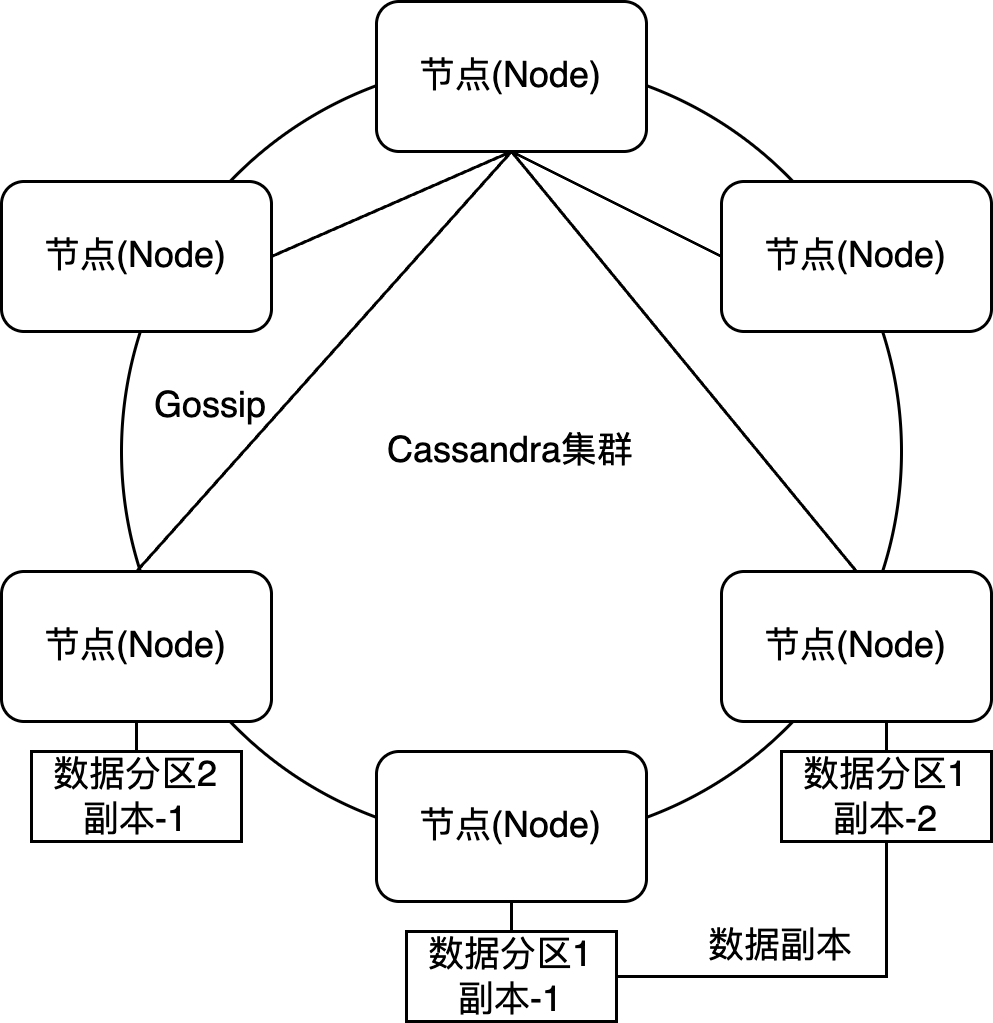
\includegraphics[width=0.5\linewidth]{cassandra-arch.png}
  \caption{Cassandra系统整体架构图}
  \label{fig:cassandra-arch}
\end{figure}

Cassandra基本组成单元是节点(Node),节点代表单个运行Cassandra进程的实例,通常运行在成本较低的商用硬件上。Cassandra集群中通常由多个节点组成。每个节点是同质性的,提供和其他节点完全相同的功能。
节点是Cassandra线性可扩展性的基础,通过增加节点进行横向扩展,Cassandra可以增加其管理的数据量、服务的吞吐量。
节点直接通过叫做Gossip的一种P2P协议进行通信。

Cassandra上管理的数据会被进一步划分为更小粒度的分区,从而在各个节点中均匀分布数据。Cassandra通过一致性哈希算法\cite{karger1997consistent}决定每个节点负责的数据范围。分区情况会被Gossip协议广播到所有节点,从而使每个节点都能够对外提供正确的服务。

Cassandra通过数据副本来保证可用性和容错能力,通过一致性协议保证副本的一致性。
Cassandra通过复制因子(RF)为同一个分区保留多个副本,保证即使一个副本宕机,其他副本仍然可以满足请求,且副本可以被放置在不同的数据中心,从而获得更高的安全性和性能。Cassandra通过一致性级别(CL)来决定操作的一致性,表示在操作被视为成功之前,必须向协调器确认读取或写入操作的最小Cassandra节点数。


\subsection{节点故障检测}

Cassandra中的每个节点通过Gossip协议来定期交换彼此的信息,并使用Phi累积性故障(Phi Accrual)检测算法\cite{hayashibara2004spl}来判断某个节点是否出现故障。

每个节点定期(通常每秒一次)通过Gossip协议选择几个节点交换彼此的状态信息,包括节点的运行状态、负载信息、该节点已知集群中其他节点的信息,使得信息可以快速有效地传播到整个集群。Gossip协议是一种最终一致性协议,随着时间的推移,所有节点最终都会收敛到一致的集群状态。

Cassandra的Phi累积性故障检测算法会根据Gossip交换的状态信息来计算出某个节点失效的可能性,避免了简单的地使用超时机制,而是通过统计分析心跳间隔,来预测节点失效的概率。Phi Accrual检测器会记录节点之间心跳信息到达的时间间隔,计算出一个“Phi”值,表示节点失效的可能性。Cassandra会设置一个Phi阈值,当Phi值超过这个阈值时,就认为节点失效。Phi Accrual检测器能够根据网络状况动态调整在网络不稳定的情况下,它会降低Phi阈值,以避免误判,在网络稳定的情况下,它会提高Phi阈值,以提高检测的准确性。在瞬态网络问题期间,节点可能暂时无法访问。使用phi accrual可以更宽容的对待这类网络问题,减少不必要的节点失效判断。


\section{TiDB系统的高可用方案}
TiDB\cite{huang2020tidb}是开源的分布式关系性数据库,同时支持OLTP和OLAP的能力,具备水平扩缩容、金融级高可用、实时 HTAP、云原生、兼容MySQL生态等优势。

\subsection{TiDB的整体架构}

TiDB集群可以划分为位于中间代理层的TiProxy,位于计算层的TiDB,和位于存储层的TiKV和TiFlash,以及集群的协调节点PD(Placement Driver)。

\begin{figure}
  \centering
  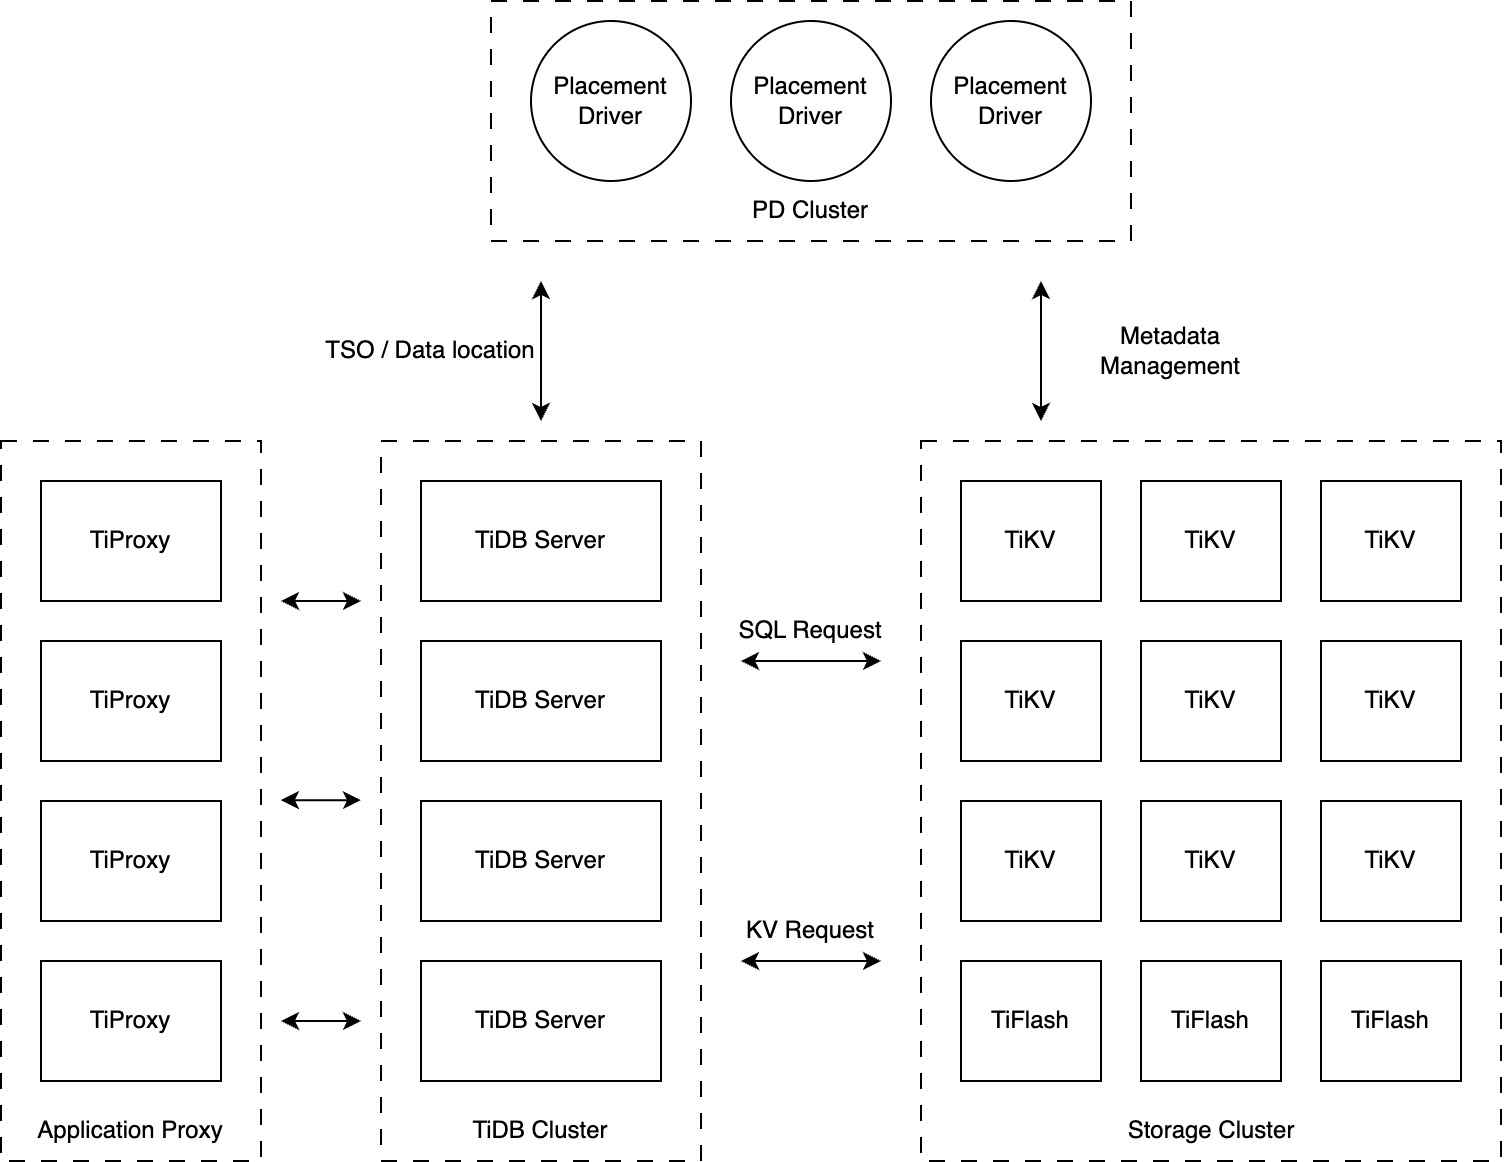
\includegraphics[width=0.9\linewidth]{tidb-arch.png}
  \caption{TiDB系统整体架构图}
  \label{fig:tidb-arch}
\end{figure}

PD(Placement Driver)是集群的大脑,负责元信息管理,实时监控和调整集群节点的整体拓扑结构、每一个节点的数据分布情况。

TiKV和TiFlash是数据的存储节点。TiKV是具备分布式事务能力的键值存储引擎,而TiFlash是为查询负载专门优化的列式存储引擎。
数据的存储以Region作为单位,包含了一段Key的区间,TiKV通过Region来实现数据分区和负载均衡,并会为每一个Region维护多个副本来服务高可用性。

TiDB是无状态的计算节点,负责接受客户端的连接,对SQL解析和优化,生成分布式执行计划,并将计划转发给存储节点进行执行。

TiProxy是部署在客户端应用和TiDB之间代理节点,提供负载均衡、连接持久化、服务发现和其他功能。


\subsection{故障的检测和发现}

在TiDB集群中,PD负责检测定期交换心跳来维持对每个节点、每个Region和集群全体的拓扑的拓扑感知,并会在检测到错误的时候尝试自动恢复。TiDB Server会通过PD获取最新的数据分区和地址,生成对应的查询计划。TiProxy会保持对TiDB Server的检测和探活。

TiKV会定期向PD发送心跳包,交换的内容包括总磁盘容量和磁盘用量、节点承载的Region数量、数据写入和读取的负载情况、发送/接受的snapshot数量等相关信息。如果PD在一段时间内没有收到TiKV的心跳,那么就会认为该节点可能出现故障,将其状态标记为异常,并且综合考虑用户配置和集群实际情况,来判断是否将该节点从集群中移除,并进行相应的调度操作,例如将该TiKV上的Region进行迁移。

每一个Region的Raft Leader也会定期向PD发送心跳包,交换的内容包括Leader所在的位置、每一个Follower所在的位置、掉线的副本个数和该Region的写入/读取速度。当Leader掉线,其他的Follower节点可能会触发新的选举,同时若PD长时间没有收到心跳,也可能触发主动的Leader切换和副本的调度。

\subsection{最高级别的容灾能力}

通过多数据副本、多机房部署、多地分布部署,TiDB集群可以实现RPO为零,RTO在一分钟以内的目标,同时容忍单节点故障、数据中心故障、一整个城市级别的灾难。以下是对TiDB的两地三中心五副本的部署结构描述:




\section{Oceanbase系统的高可用方案}

Oceanbase是开源的分布式关系性数据库,兼具分布式架构的扩展性和集中式架构的性能优势,过单一引擎支持混合事务/分析处理(HTAP),具备强数据一致性、高可用性、高性能、在线扩展、与 SQL 和主流关系型数据库的高度兼容性等优势。

\subsection{Oceanbase的整体架构}

Oceanbase集群主要包括OBServer和OBProxy两个角色。每一个OBServer上都运行着Oceanbase的一个进程,内部可进一步细分为根服务(Root Service)、SQL引擎、事务引擎和存储引擎。OBProxy则充当中间层,接收来自应用程序的SQL请求将其路由到集群内最佳的OBServer节点,然后将执行结果返回给应用程序。

\begin{figure}
  \centering
  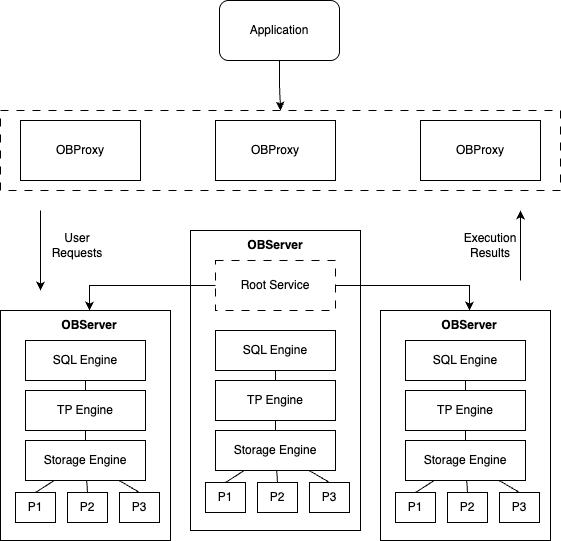
\includegraphics[width=0.9\linewidth]{oceanbase-arch.png}
  \caption{Oceanbase系统整体架构图}
  \label{fig:oceanbase-arch}
\end{figure}

根服务是集成在Oceanbase进程内的逻辑服务,负责维护集群的元数据,包括表结构、分区信息、节点状态等。根服务会通过心跳机制检测每一个OBServer的健康状况,如果发现故障,则会触发恢复流程,包括重新选举领导者或重新复制分区。根服务还会负责监控集群的负载情况,会进行分区移动、分区复制和领导者切换等操作,以确保各个节点的资源利用率均衡。

OBServer还包含了SQL引擎,用于接受用户请求并生成对应的计划,以及基于LSM结构的存储引擎。

集群内的元数据和用户数据都是以分区的方式进行水平划分和存储,并通过副本复制的方式保证分区的高可用。Oceanbase采用了基于哈希和范围的双层划分算法,但会保证同一个表组的分区被分配在同一个节点上。Oceanbase采用Paxos对每一个分区的redo log进行复制管理,在故障恢复的时候,通过重放redo log实现恢复。

OBProxy 用于将请求路由到 OBServer。当接收到用户的 SQL 查询时,OBProxy 将解析该查询,然后根据分区的位置信息将查询发送到相应的 OBServer,提供服务发现和负载均衡等能力。


\subsection{Oceanbase的快速故障发现}

OceanBase通过校验和、针对Paxos恢复和选举优化、基于RPC机制的节点检测等方式尽可能提前错误发生的时间。

在校验和上,Oceanbase在每次从磁盘中读写数据的时候都会计算和比较校验和,在每次大合并之后对每一个数据分区的副本重新比对校验和,在重放Redo Log的时候会计算每一条事务的累积校验和。通过事务粒度的校验和机制,Oceanbase能够发现软件实现中事务处理和并发控制两个模块的人为程序漏洞。

在Paxos算法上,Oceanbase通过大幅减少故障单元和稳定的选举算法来提高故障的发现能力。
在前文所提到的TiDB中,故障恢复单元是每一个Raft组。当上层业务的分区特别多、单一节点上承载的Raft数量特别多的情况下,故障恢复的单元数量就会水平扩张,量级巨大。然而,在Oceanbase 4.0版本之后,故障恢复的单元转变成一个单机的日志流,在逻辑上可以把每一个节点视作一个整体的Paxos组,因此故障恢复单元将不再和业务的元数据和实际数据量有关,从而进一步降低了故障恢复的复杂性和时间。
传统的Paxos选举流程基于随机算法,并且依赖节点之间的时钟同步,例如NTP。Oceanbase的实现消除了对节点间时钟同步的依赖,完全基于消息驱动,依靠节点之间的消息交互和顺序来触发选举,并激进地将Leader的Lease时间缩短到了4s以内,从而能够更快地检测到故障并完成新的Leader选举。

Oceanbase 4.0中,节点间健康状态监测机制从基于TCP的连接机制转变为基于RPC框架内部的方式。3.0版本中OceanBase采用定期发送TCP Keepalive的探测包来检测节点之间的网络连接是否正常,然而这种检测只能用于判断网络情况,如果OBServer进程出现问题(例如Coredump崩溃),但TCP连接依然存在,KeepAlive机制无法识别。因此,在4.0版本中,Oceanbase框架内值了健康状态监测机制,通过定期发送应用程序级别的心跳包,从而能同时监测网络和进程的健康。同时,由于RPC 框架内部的检测机制能够检测应用程序的响应延迟、错误率等指标,从而提供更细粒度的健康状态信息。

\subsection{Oceanbase的故障恢复和Client协同}

Oceanbase通过Paxos并行回放、故障时期领导指定、Client的建连探活等方式提高故障恢复的速度。

在前一节所述,Oceanbase的故障恢复单元是一个单一的Paxos Group,为了提高故障恢复的速度,Oceanbase需要进行并行、实时地回放日志中的事务,从而防止日志回放成为性能的瓶颈。在Oceanbase中,不同事务的Redo日志可以并行回放,同一事物的不同Redo日志也可以并行回放,通过事务的ID


\section{插图}

图片通常在 \env{figure} 环境中使用 \cs{includegraphics} 插入,如图~\ref{fig:example} 的源代码。
建议矢量图片使用 PDF 格式,比如数据可视化的绘图;
照片应使用 JPG 格式;
其他的栅格图应使用无损的 PNG 格式。
注意,LaTeX 不支持 TIFF 格式;EPS 格式已经过时。

\begin{figure}
  \centering
  \includegraphics[width=0.5\linewidth]{example-image-a.pdf}
  \caption*{国外的期刊习惯将图表的标题和说明文字写成一段,需要改写为标题只含图表的名称,其他说明文字以注释方式写在图表下方,或者写在正文中。}
  \caption{示例图片标题}
  \label{fig:example}
\end{figure}

若图或表中有附注,采用英文小写字母顺序编号,附注写在图或表的下方。
国外的期刊习惯将图表的标题和说明文字写成一段,需要改写为标题只含图表的名称,其他说明文字以注释方式写在图表下方,或者写在正文中。

如果一个图由两个或两个以上分图组成时,各分图分别以 (a)、(b)、(c)...... 作为图序,并须有分图题。
推荐使用 \pkg{subcaption} 宏包来处理, 比如图~\ref{fig:subfig-a} 和图~\ref{fig:subfig-b}。

\begin{figure}
  \centering
  \subcaptionbox{分图 A\label{fig:subfig-a}}
    {\includegraphics[width=0.35\linewidth]{example-image-a.pdf}}
  \subcaptionbox{分图 B\label{fig:subfig-b}}
    {\includegraphics[width=0.35\linewidth]{example-image-b.pdf}}
  \caption{多个分图的示例}
  \label{fig:multi-image}
\end{figure}



\section{表格}

表应具有自明性。为使表格简洁易读,尽可能采用三线表,如表~\ref{tab:three-line}。
三条线可以使用 \pkg{booktabs} 宏包提供的命令生成。

\begin{table}
  \centering
  \caption{三线表示例}
  \begin{tabular}{ll}
    \toprule
    文件名          & 描述                         \\
    \midrule
    thuthesis.dtx   & 模板的源文件,包括文档和注释 \\
    thuthesis.cls   & 模板文件                     \\
    thuthesis-*.bst & BibTeX 参考文献表样式文件    \\
    \bottomrule
  \end{tabular}
  \label{tab:three-line}
\end{table}

表格如果有附注,尤其是需要在表格中进行标注时,可以使用 \pkg{threeparttable} 宏包。
研究生要求使用英文小写字母 a、b、c……顺序编号,本科生使用圈码 ①、②、③……编号。

\begin{table}
  \centering
  \begin{threeparttable}[c]
    \caption{带附注的表格示例}
    \label{tab:three-part-table}
    \begin{tabular}{ll}
      \toprule
      文件名                 & 描述                         \\
      \midrule
      thuthesis.dtx\tnote{a} & 模板的源文件,包括文档和注释 \\
      thuthesis.cls\tnote{b} & 模板文件                     \\
      thuthesis-*.bst        & BibTeX 参考文献表样式文件    \\
      \bottomrule
    \end{tabular}
    \begin{tablenotes}
      \item [a] 可以通过 xelatex 编译生成模板的使用说明文档;
        使用 xetex 编译 \file{thuthesis.ins} 时则会从 \file{.dtx} 中去除掉文档和注释,得到精简的 \file{.cls} 文件。
      \item [b] 更新模板时,一定要记得编译生成 \file{.cls} 文件,否则编译论文时载入的依然是旧版的模板。
    \end{tablenotes}
  \end{threeparttable}
\end{table}

如某个表需要转页接排,可以使用 \pkg{longtable} 宏包,需要在随后的各页上重复表的编号。
编号后跟表题(可省略)和“(续)”,置于表上方。续表均应重复表头。

\begin{longtable}{cccc}
    \caption{跨页长表格的表题}
    \label{tab:longtable} \\
    \toprule
    表头 1 & 表头 2 & 表头 3 & 表头 4 \\
    \midrule
  \endfirsthead
    \caption*{续表~\thetable\quad 跨页长表格的表题} \\
    \toprule
    表头 1 & 表头 2 & 表头 3 & 表头 4 \\
    \midrule
  \endhead
    \bottomrule
  \endfoot
  Row 1  & & & \\
  Row 2  & & & \\
  Row 3  & & & \\
  Row 4  & & & \\
  Row 5  & & & \\
  Row 6  & & & \\
  Row 7  & & & \\
  Row 8  & & & \\
  Row 9  & & & \\
  Row 10 & & & \\
\end{longtable}



\section{算法}

算法环境可以使用 \pkg{algorithms} 或者 \pkg{algorithm2e} 宏包。

\renewcommand{\algorithmicrequire}{\textbf{输入:}\unskip}
\renewcommand{\algorithmicensure}{\textbf{输出:}\unskip}

\begin{algorithm}
  \caption{Calculate $y = x^n$}
  \label{alg1}
  \small
  \begin{algorithmic}
    \REQUIRE $n \geq 0$
    \ENSURE $y = x^n$

    \STATE $y \leftarrow 1$
    \STATE $X \leftarrow x$
    \STATE $N \leftarrow n$

    \WHILE{$N \neq 0$}
      \IF{$N$ is even}
        \STATE $X \leftarrow X \times X$
        \STATE $N \leftarrow N / 2$
      \ELSE[$N$ is odd]
        \STATE $y \leftarrow y \times X$
        \STATE $N \leftarrow N - 1$
      \ENDIF
    \ENDWHILE
  \end{algorithmic}
\end{algorithm}
